\chapter{Verknüpfungsschaltungen}

\section{Einführung}

Logische Verknüpfungsschaltungen sind das Grundgerüst der digitalen Technik. Mit Hilfe der 5 hier aufgeführten Verknüpfungsschaltungen, die auch Gatter genannt werden, lassen sich nun alle anderen Verknüpfungsschaltungen realisieren.\index{Verknüpfungsschaltungen}\index{Gatter}

Die Wahrheitstabelle, oder auch Logik-Tafel, die bei jeder Verknüpfungsschaltung mit aufgeführt wird, gibt an, welches Signal am Ausgang anliegt, nachdem die Eingänge in einer bestimmten Weise angeschlossen wurden. Dabei werden alle möglichen Anschlusskombinationen durchgespielt.\index{Wahrheitstabelle}

\section{AND-Gatter (UND-Verknüpfung)}

Die Boolesche Funktionsgleichung (mathematische Gleichung) für das AND-Gatter lautet:\index{AND}\index{Gatter}

\begin{quote}
  A = E\textsubscript{1} \ensuremath{\wedge} E\textsubscript{2}  (sprich: „E\textsubscript{1} und E\textsubscript{2}“)
\end{quote}


Das bedeutet, dass A nur dann den Wert 1 hat, wenn die Eingänge E\textsubscript{1} und E\textsubscript{2} den Wert 1 haben. In allen anderen Fällen hat der Ausgang A den Wert 0. Anhand der Logik-Tafel ist dies leicht zu erkennen. In der Zeile, in der A den Wert 1 hat, haben die beiden Eingänge ebenfalls den Wert 1.

\begin{table}[htbp]
  \centering
  \caption{Logiktafel AND-Gatter}
  \begin{tabular}{ccc}
    \toprule
    E\textsubscript{1} & E\textsubscript{2} & A \\
    \midrule
    0 & 0 & 0 \\
    0 & 1 & 0 \\
    1 & 0 & 0 \\
    1 & 1 & 1 \\
    \bottomrule
  \end{tabular}
\end{table}

\begin{figure}[htbp]
  \centering
  
\includegraphics[width=.8\linewidth]{media/abb-04}
  \caption{Schaltsymbol AND}
\end{figure}

Hier ist die einfachste UND-Verknüpfung gewählt worden, nämlich die mit 2 Eingängen. Tatsächlich gibt es jedoch auch AND-Gatter mit mehr  als zwei Eingängen. Die mathematische Logik bleibt dabei aber gleich: Nur wenn alle Eingänge den Wert 1 haben, hat der Ausgang ebenfalls den Wert 1.\index{AND}\index{Gatter}

Die UND-Verknüpfung wird auch als „Konjunktion“ bezeichnet, was so viel heißt wie „Bindung“.\index{Konjunktion}

\section{OR-Gatter (ODER-Verknüpfung)}

Hier heißt die mathematischer Gleichung:

\begin{quote}
  A = E1 \ensuremath{\vee} E2  (sprich: „E1 oder E2“)
\end{quote}


Dabei hat A dann den Wert 1, wenn E\textsubscript{1} oder E\textsubscript{2} oder beide (!) Eingänge den Wert 1 haben. Dieses Verhalten unterscheidet sich von dem normalen Sprachgebrauch des Wortes „oder“. Hier bedeutet es: A hat nur dann den Wert 0, wenn beide Eingänge den Wert 0 haben. Sonst hat der Ausgang den Wert 1.

\begin{table}[htbp]
  \centering
  \caption{Logiktafle OR-Gatter}
  \begin{tabular}{ccc}
    \toprule
    E\textsubscript{1} & E\textsubscript{2} & A \\
    \midrule
    0 & 0 & 0 \\
    0 & 1 & 1 \\
    1 & 0 & 1 \\
    1 & 1 & 1 \\
    \bottomrule
  \end{tabular}
\end{table}

\begin{figure}[htbp]
  \centering
  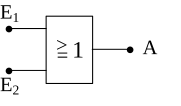
\includegraphics[width=.8\linewidth]{media/abb-05}
  \caption{Schaltsymbol OR}
\end{figure}

Die ODER-Verknüpfung gibt es ebenfalls mit mehr als zwei Eingängen, wobei sich die mathematischer Logik wie beim AND-Gatter nicht ändert. Eine andere Bezeichnung für das OR-Gatter ist die „Disjunktion“, das heißt „Trennung“.\index{ODER-Verknüpfung}\index{AND}\index{Gatter}\index{OR-Gatter}\index{Disjunktion}

\section{INVERTER (NOT-Verknüpfung)}

Das Schaltsymbol des Inverters ist unten abgebildet. Dabei lässt sich die mathematische Logik durch folgende Gleichung darstellen:\index{Inverters}

\begin{quote}
  A = \ensuremath{\lnot}E (sprich „E komplementär“ oder „E negiert“).
\end{quote}
\index{komplementär}

\begin{table}[htbp]
  \centering
  \caption{Logiktafel NOT-Gatter}
  \begin{tabular}{cc}
    \toprule
    E & A \\
    \midrule
    0 & 1 \\
    1 & 0 \\
    \bottomrule
  \end{tabular}
\end{table}

\begin{figure}[htbp]
  \centering
  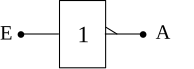
\includegraphics[width=.8\linewidth]{media/abb-06}
  \caption{Schaltsymbol NOT}
\end{figure}

Ein anderer Begriff für den Inverter ist die „Negation“. Indem man nun das AND-Gatter und das OR-Gatter negiert, erhält man zwei weitere wichtige Verknüpfungsschaltungen.\index{Negation}\index{AND}\index{Gatter}\index{OR-Gatter}\index{Verknüpfungsschaltungen}

\section{NAND-Gatter}

Gebildet aus den englischen Worten „not and“, also „nicht und“. Daraus lässt sich bereits schließen, dass die Verknüpfung negiert sein muss. Die mathematische Gleichung bestätigt dies:

\begin{quote}
  A = \ensuremath{\lnot}(E\textsubscript{1} \ensuremath{\wedge} E\textsubscript{2}) (sprich: „E\textsubscript{1} und E\textsubscript{2} negiert“)
\end{quote}


Der Ausgang A hat immer den Wert 1, außer wenn beide Eingänge den Wert 1 haben. Anhand der Logik-Tafel lässt sich auch erkennen, dass die NAND-Funktion an ihrem Ausgang genau das entgegengesetzte Signal hat wie das AND-Gatter.\index{AND}\index{Gatter}

\begin{table}[htbp]
  \centering
  \caption{Logiktafel NAND-Gatter}
  \begin{tabular}{ccc}
    \toprule
    E\textsubscript{1} & E\textsubscript{2} & A \\
    \midrule
    0 & 0 & 1 \\
    0 & 1 & 1 \\
    1 & 0 & 1 \\
    1 & 1 & 0 \\
    \bottomrule
  \end{tabular}
\end{table}

\begin{figure}[htbp]
  \centering
  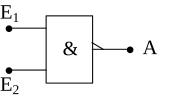
\includegraphics[width=.8\linewidth]{media/abb-07}
  \caption{Schaltsymbol NAND}
\end{figure}

\section{NOR-Gatter}

Gebildet aus den englischen Wörtern „not or“, was übersetzt „nicht oder“ heißt. Es handelt sich also wiederum um eine Negation, nämlich die der OR-Verknüpfung. Die mathematische Gleichung lautet:\index{Negation}

A = \ensuremath{\lnot}(E\textsubscript{1} \ensuremath{\vee} E\textsubscript{2}) (sprich: „E\textsubscript{1} oder E\textsubscript{2} negiert“)

Bei dieser Verknüpfungsschaltung hat der Ausgang A den Wert 1, wenn beide Eingänge den Wert 0 haben. In allen anderen Fällen hat der Ausgang den Wert 0.

\begin{table}[htbp]
  \centering
  \caption{Logiktafle NOR-Gatter}
  \begin{tabular}{ccc}
    \toprule
    E\textsubscript{1} & E\textsubscript{2} & A \\
    \midrule
    0 & 0 & 1 \\
    0 & 1 & 0 \\
    1 & 0 & 0 \\
    1 & 1 & 0 \\
    \bottomrule
  \end{tabular}
\end{table}

\begin{figure}[htbp]
  \centering
  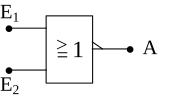
\includegraphics[width=.8\linewidth]{media/abb-08}
  \caption{Schaltsymbol NOR}
\end{figure}

Da diese beiden letzten Gatter sehr häufig vorkommen, haben sie ein eigenes Schaltsymbol. Außerdem sind sie für den Praktiker sehr interessant, da sie gegenüber den UND- bzw. ODER-Gattern meist erheblich billiger sind. Deshalb nimmt man häufig zwei NAND-Gatter um ein UND-Gatter billig aufzubauen, oder zwei NOR-Gatter für ein OR-Gatter. Die dafür notwendigen Schaltungen werden im Folgenden erklärt.\index{NAND-Gatter}\index{OR-Gatter}

\begin{figure}[htbp]
  \centering
  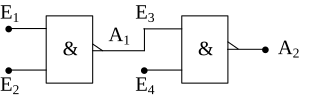
\includegraphics[width=.8\linewidth]{media/abb-09}
  \caption{Schaltbild UND-Gatter aus zwei NAND-Gatter}
\end{figure}

Bei dieser Schaltung hat der Ausgang A\textsubscript{1} nur dann den Wert 0, wenn beide Eingänge, also E\textsubscript{1} und E\textsubscript{2 }den Wert 1 haben. Der offene (nicht angeschlossene) Eingang E\textsubscript{4} hat generell den Wert 1. Um aber am Ausgang A\textsubscript{2} den Wert 1 zu erreichen, muss deswegen E\textsubscript{3} und somit am Ausgang A\textsubscript{1} der Wert 0 anliegen. Dies wird, wie oben schon beschrieben, nur dadurch erreicht, dass man den Eingängen E\textsubscript{1} und E\textsubscript{2} den Wert 1 zuordnet.

Mathematisch ausgedrückt bedeutet dies:

\begin{quote}
  A\textsubscript{1} = \ensuremath{\lnot}(E\textsubscript{1 }\ensuremath{\wedge} E\textsubscript{2})
\end{quote}


\begin{quote}
  A\textsubscript{2} = \ensuremath{\lnot}A\textsubscript{1} = \ensuremath{\lnot}(\ensuremath{\lnot}(E\textsubscript{1 }\ensuremath{\wedge} E\textsubscript{2}))
\end{quote}


\ensuremath{\lnot}(\ensuremath{\lnot}(E\textsubscript{1 }\ensuremath{\wedge} E\textsubscript{2})) ist aber nichts anderes als E\textsubscript{1 }\ensuremath{\wedge} E\textsubscript{2}; somit gilt die Funktionsgleichung der normalen UND-Verknüpfung:

\begin{quote}
  A\textsubscript{2} = E\textsubscript{1 }\ensuremath{\wedge} E\textsubscript{2}
\end{quote}


Dies beweist, dass die obige Schaltung einer normalen UND-Verknüpfung entspricht.

\begin{figure}[htbp]
  \centering
  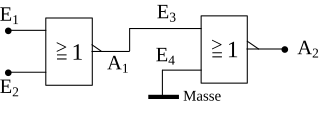
\includegraphics[width=.8\linewidth]{media/abb-10}
  \caption{Schaltbild OR-Gatter aus zwei NOR-Gatter}
\end{figure}

Die Logik dieser Schaltung ist ähnlich der Vorherigen. Der Ausgang A\textsubscript{2} hat nur dann den Wert 0, wenn E\textsubscript{3} den Wert 1 hat. E\textsubscript{4} ist durch den Masseanschluss sowieso immer auf 0. Der Wert 1 an E\textsubscript{3} und somit an A\textsubscript{1} wird aber nur erreicht, indem man E\textsubscript{1} und E\textsubscript{2} den Wert 0 zuordnet. In allen anderen Fällen hat A\textsubscript{1} den Wert 0 und damit A\textsubscript{2} den Wert 1. Dies wiederum entspricht genau der OR-Verknüpfung.\index{Masseanschluss}

Hier der mathematische Beweis:

\begin{quote}
  A\textsubscript{1} = \ensuremath{\lnot}(E\textsubscript{1 }\ensuremath{\vee} E\textsubscript{2})
\end{quote}


\begin{quote}
  A\textsubscript{2} = \ensuremath{\lnot}A\textsubscript{1} = \ensuremath{\lnot}(\ensuremath{\lnot}(E\textsubscript{1 }\ensuremath{\vee} E\textsubscript{2})) = E\textsubscript{1 }\ensuremath{\vee} E\textsubscript{2}
\end{quote}


Mit diesen nun beschriebenen 5 Grundschaltungen (AND-, NAND-, OR-, NOR-Gatter und Inverter) lassen sich alle anderen logischen Verknüpfungsschaltungen realisieren. Man muss nur die gewünschten Elemente zusammenschalten. Den mathematischen Hintergrund für die Kombination der Gatter liefert die Boolesche Algebra. Die Grundfunktionen sind bei der Erklärung der Schaltungen mit angegeben.\index{Grundschaltungen}\index{Verknüpfungsschaltungen}

\section{EX-OR-Gatter (Exklusiv-ODER)}

Eine Variation der Zusammenschaltung der 5 Grundgatter ist das Exklusiv-ODER. Im Gegensatz zur ODER-Verknüpfung tritt am Ausgang nicht der Wert 1 auf, wenn beide Eingänge den Wert 1 haben. Diese Funktion entspricht jetzt dem „oder“ wie es im normalen Sprachgebrauch verwendet wird. Das heißt, dass am Ausgang der Wert 1 vorliegt, wenn E\textsubscript{1} oder E\textsubscript{2} den Wert 1 haben. Sobald E\textsubscript{1} und E\textsubscript{2} den gleichen Wert haben, liegt am Ausgang A der Wert 0.\index{Exklusiv-ODER}\index{ODER-Verknüpfung}

\begin{table}[htbp]
  \centering
  \caption{Logiktafel Ex-OR-Gatter}
  \begin{tabular}{ccc}
    \toprule
    E\textsubscript{1} & E\textsubscript{2} & A \\
    \midrule
    0 & 0 & 0 \\
    0 & 1 & 1 \\
    1 & 0 & 1 \\
    1 & 1 & 0 \\
    \bottomrule
  \end{tabular}
\end{table}

\begin{figure}[htbp]
  \centering
  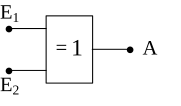
\includegraphics[width=.8\linewidth]{media/abb-11}
  \caption{Schaltsymbol EX-OR-Gatter}
\end{figure}

Da diese Verknüpfungsschaltung sehr häufig vorkommt, hat auch sie ihr eigenes Schaltsymbol. Sie kann aber auch durch die Zusammenschaltung von 2 Invertern, 2 AND-Gattern und einem NOR-Gatter aufgebaut werden. Die mathematische Funktion lautet:

\begin{quote}
  A = (\ensuremath{\lnot}E\textsubscript{1} \ensuremath{\wedge} E\textsubscript{2}) \ensuremath{\vee} (E\textsubscript{1} \ensuremath{\wedge} \ensuremath{\lnot}E\textsubscript{2})
\end{quote}


Nun zum Schaltbild des Exklusiv-ODER. Ein Praktiker kann schon anhand der mathematischen Gleichung das Schaltbild zeichnen. Man muss dabei nur genau die Gleichung in die Schaltsymbole der logischen Verknüpfung umwandeln.\index{Exklusiv-ODER}

\begin{figure}[htbp]
  \centering
  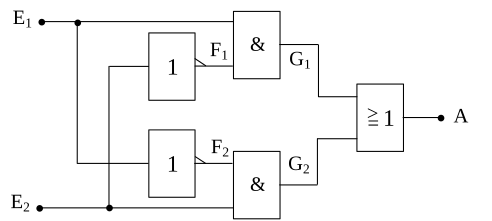
\includegraphics[width=.8\linewidth]{media/abb-12}
  \caption{Schaltbild EX-OR-Gatter}
\end{figure}

Bei dieser Schaltung wollen wir nun einmal einen anderen Weg gehen, der sich vor allem bei komplexen und komplizierteren Schaltungen als sehr einfach herausstellt. Dabei wird an die beiden Eingänge E\textsubscript{1} und E\textsubscript{2} jede mögliche Eingangskombination gelegt und bis zum Ausgang A „durchgespielt“. Im vorliegenden Fall sind das genau 4 Kombinationen.

An E\textsubscript{1} und E\textsubscript{2} liegt jeweils der Wert 0. Das obere AND-Gatter hat also am Eingang den Wert 0 von E\textsubscript{1} und den Wert 1 vom invertierten E\textsubscript{2}. Das ergibt einen Zwischenwert G\textsubscript{1} = 0. Das untere AND-Gatter hat ebenfalls den Wert 0 (von E\textsubscript{2}) und den Wert 1 (invertiertes E\textsubscript{1}) und somit ebenfalls den Zwischenwert G\textsubscript{2} = 0. Diese beiden Zwischenwerte liegen nun an einem OR-GATTER, das dadurch am Ausgang den Wert 0 hat. Damit ist die erste Zeile der Logik-Tafel schon festgelegt.\index{AND}\index{AND-Gatter}

Nun legt man an E\textsubscript{1} den Wert 0 und an E\textsubscript{2} den Wert 1. Da E\textsubscript{2} invertiert an das obere AND-Gatter gelangt und E\textsubscript{1} von vorneherein 0 ist, erscheint am oberen Zwischenausgang G\textsubscript{1} der Wert 0. Beim unteren AND-Gatter sind dagegen beide Eingänge auf dem Wert 1, da E\textsubscript{1} invertiert wird und E\textsubscript{2} den Wert 1 hat. Das ergibt am Zwischenausgang G\textsubscript{2} den Wert 1. Am OR-Gatter liegt also nun einmal der Wert 0 (G\textsubscript{1}) und einmal der Wert 1 (G\textsubscript{2}). Der Ausgang A hat somit den Wert 1.\index{AND}\index{AND-Gatter}\index{OR-Gatter}

Wenn man nun an den Eingang E\textsubscript{1} den Wert 1 und an E\textsubscript{2} den Wert 0 legt, so läuft die Logik genau den gleichen Weg. Nur liegen dabei die Werte die vorher am oberen AND-Gatter lagen nun am unteren und umgekehrt. Am Ausgang erscheint deshalb wie unter 2. der Wert 1.\index{AND}

Die letzte Kombinationsmöglichkeit ist nun die, dass beide Eingänge E\textsubscript{1} und E\textsubscript{2} den Wert 1 bekommen. Durch die Invertierung von E\textsubscript{2} am oberen und E\textsubscript{1} am unteren AND-Gatter haben die Zwischenausgänge G\textsubscript{1} und G\textsubscript{2} die gleichen Werte, nämlich 0. Eine Parallele dazu ist die erste Kombination. Am Ausgang A erscheint deshalb der Wert 0.\index{AND}

\section{EX-NOR-Gatter}

Eine Variation des EX-OR-Gatters ist diese Schaltung. Dabei wird nur der Ausgang A der oberen Schaltung invertiert.

\begin{table}[htbp]
  \centering
  \caption{Logiktafel EX-NOR-Gatter}
  \begin{tabular}{ccc}
    \toprule
    E\textsubscript{1} & E\textsubscript{2} & A \\
    \midrule
    0 & 0 & 1 \\
    0 & 1 & 0 \\
    1 & 0 & 0 \\
    1 & 1 & 1 \\
    \bottomrule
  \end{tabular}
\end{table}

\begin{figure}[htbp]
  \centering
  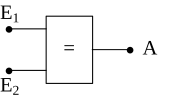
\includegraphics[width=.8\linewidth]{media/abb-13}
  \caption{Schaltsymbol EX-NOR-Gatter}
\end{figure}

\begin{figure}[htbp]
  \centering
  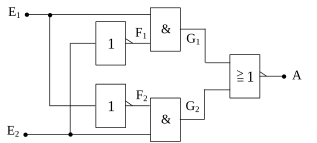
\includegraphics[width=.8\linewidth]{media/abb-14}
  \caption{Schaltbild EX-NOR-Gatter}
\end{figure}

\section{Gatter mit mehreren Eingängen}

Oftmals ist es nötig, Verknüpfungsschaltungen mit 3 oder 4 Eingängen in eine Schaltung zu integrieren. Haben Sie diese Gatter nicht zur Hand, so kann man sie mit den unten abgebildeten Schaltungen aufbauen.\index{Verknüpfungsschaltungen}\index{Gatter}

Zuerst die AND-Verknüpfung mit 3 Eingängen. Die folgende Tabelle zeigt, dass die abgebildete Schaltung einem AND-Gatter mit 3 Eingängen entspricht. Eingezeichnet sind auch die Zwischenausgänge Z\textsubscript{1}, Z\textsubscript{2} und Z\textsubscript{3}.

\begin{table}[htbp]
  \centering
  \begin{tabular}{ccccccc}
    \toprule
    E\textsubscript{1} & E\textsubscript{2} & E\textsubscript{3} & Z\textsubscript{1} & Z\textsubscript{2} & Z\textsubscript{3} & A \\
    \midrule
    0 & 0 & 0 & 1 & 0 & 1 & 0 \\
    0 & 0 & 1 & 1 & 0 & 1 & 0 \\
    0 & 1 & 0 & 1 & 0 & 1 & 0 \\
    0 & 1 & 1 & 1 & 0 & 1 & 0 \\
    1 & 0 & 0 & 1 & 0 & 1 & 0 \\
    1 & 0 & 1 & 1 & 0 & 1 & 0 \\
    1 & 1 & 0 & 0 & 1 & 1 & 0 \\
    1 & 1 & 1 & 0 & 1 & 0 & 1 \\
    \bottomrule
  \end{tabular}
\end{table}

\begin{figure}[htbp]
  \centering
  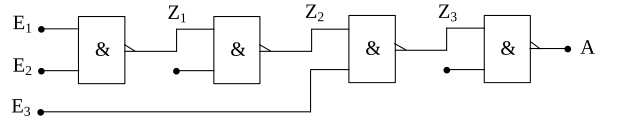
\includegraphics[width=.8\linewidth]{media/abb-15}
  \caption{Schaltbild AND-Gatter mit 3 Eingänge aus NAND-Gattern}
\end{figure}

Nach diesem Schema lässt sich auch eine UND-Schaltung mit 4 Eingängen aus 6 NAND-Gattern aufbauen usw.

NOR-Gatter mir 3 Eingängen aus 3 NOR-Gattern

Die folgende Logiktafel mit den Zwischenausgängen gibt auch hier wiederum Auskunft darüber, dass das Verhalten der Schaltung dem eines NOR-Gatters mit 3 Eingängen entspricht.

\begin{table}[htbp]
  \centering
  \begin{tabular}{cccccc}
    \toprule
    E\textsubscript{1} & E\textsubscript{2} & E\textsubscript{3} & Z\textsubscript{1} & Z\textsubscript{2} & A \\
    \midrule
    0 & 0 & 0 & 1 & 0 & 1 \\
    0 & 0 & 1 & 1 & 0 & 0 \\
    0 & 1 & 0 & 0 & 1 & 0 \\
    0 & 1 & 1 & 0 & 1 & 0 \\
    1 & 0 & 0 & 0 & 1 & 0 \\
    1 & 0 & 1 & 0 & 1 & 0 \\
    1 & 1 & 0 & 0 & 1 & 0 \\
    1 & 1 & 1 & 0 & 1 & 0 \\
    \bottomrule
  \end{tabular}
\end{table}

\begin{figure}[htbp]
  \centering
  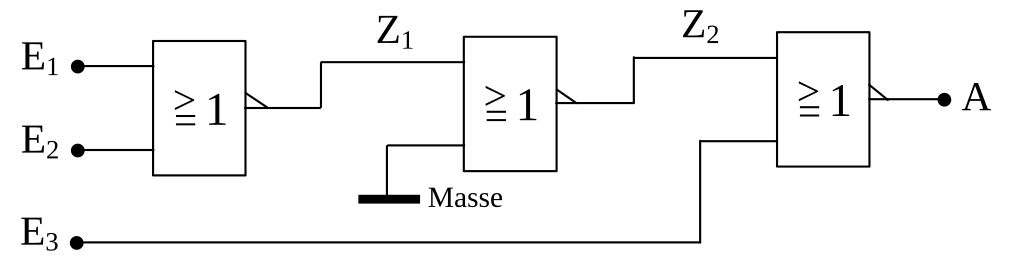
\includegraphics[width=.8\linewidth]{media/abb-16}
  \caption{Schaltbild NOR-Gatter mit 3 Eingängen aus 3 NOR-Gatter}
\end{figure}

Auch bei dieser Schaltung lassen sich durch Hinzufügen weiterer NOR-Gatter Schaltungen erzeugen, die sich wie große NOR-Gatter mit noch mehr Eingängen verhalten.

\section{Kombi-Schaltungen}

Neben den bisher gezeigten Verknüpfungsschaltungen gibt es noch weitere Schaltsymbole für spezielle Kombinationen. Daher der Name Kombi-Schaltungen. Sie werden in dieser Form sehr häufig für Decoder und andere logische Schaltungen benötigt. Aus diesem Grunde hat man auch für sie vereinfachte Darstellungen gefunden.\index{Verknüpfungsschaltungen}

1. Zwei OR-Gatter, deren Ausgänge über ein AND-Gatter verknüpft sind:\index{AND-Gatter}

\begin{figure}[htbp]
  \centering
  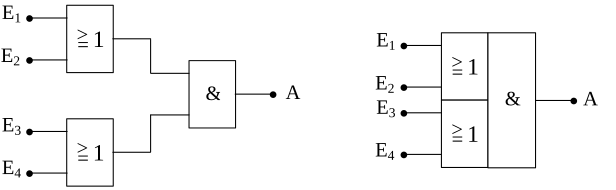
\includegraphics[width=.8\linewidth]{media/abb-17}
  \caption{Schaltbild Kombischaltung OR/AND}
\end{figure}

\textbf{2. AND}\textbf{-Gatter, das mit einem OR-Gatter}\textbf{ verknüpft ist:}\index{AND}\index{OR-Gatter}

\begin{figure}[htbp]
  \centering
  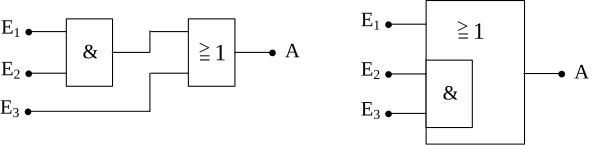
\includegraphics[width=.8\linewidth]{media/abb-18}
  \caption{Schaltbild Kombischaltung AND/OR}
\end{figure}

\textbf{3. AND-Gatter verknüpft mit einem OR-Gatter}\textbf{ (3 Eingänge) und nachgeschaltetem AND-Gatter}\index{OR-Gatter}\index{AND-Gatter}

\begin{figure}[htbp]
  \centering
  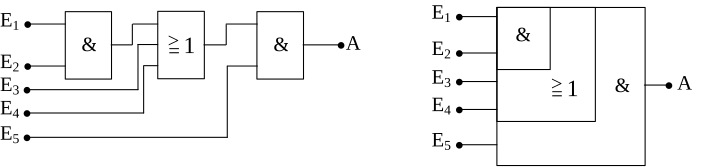
\includegraphics[width=.8\linewidth]{media/abb-19}
  \caption{Schaltbild Kombischaltung AND/NOR/AND}
\end{figure}

4. Zwei AND-Gatter, deren Ausgänge durch ein OR-Gatter miteinander verknüpft sind:\index{OR-Gatter}

\begin{figure}[htbp]
  \centering
  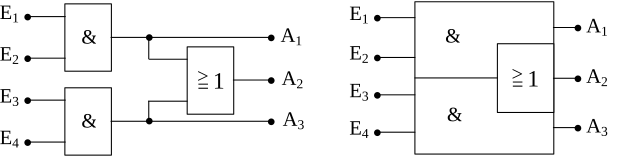
\includegraphics[width=.8\linewidth]{media/abb-20}
  \caption{Schaltbild Kombischaltung AND/NOR}
\end{figure}

